\documentclass[tikz,margin=3mm]{standalone}
\usepackage[utf8]{inputenc}
\usepackage[T1]{fontenc}
\usepackage{tikz}
\usetikzlibrary{shapes.geometric, arrows.meta, positioning, calc, fit, backgrounds}
\usepackage{xcolor}
\definecolor{primary}{HTML}{1B75BC}
\definecolor{secondary}{HTML}{F15A29}
\definecolor{accent}{HTML}{8CC63F}
\definecolor{grayC}{HTML}{4D4D4D}
\definecolor{graylight}{HTML}{F2F2F2}
\definecolor{blueC}{HTML}{1B75BC}
\definecolor{orangeC}{HTML}{F15A29}
\definecolor{yellowC}{HTML}{FBB03B}
\definecolor{purpleC}{HTML}{92278F}

\tikzset{
  base/.style={rectangle, rounded corners=4pt, draw=grayC, minimum width=3.5cm, minimum height=1cm, align=center, font=\footnotesize, fill=white, line width=0.8pt},
  ndBlue/.style={base, draw=blueC, fill=blueC!8, text=primary},
  ndOrange/.style={base, draw=orangeC, fill=orangeC!8, text=primary},
  ndGreen/.style={base, draw=accent, fill=accent!8, text=primary},
  ndYellow/.style={base, draw=yellowC, fill=yellowC!8, text=primary},
  ndPurple/.style={base, draw=purpleC, fill=purpleC!8, text=primary},
  db/.style={cylinder, draw=grayC, shape border rotate=90, aspect=0.25, fill=graylight, minimum width=2.5cm, minimum height=1.5cm, align=center, font=\footnotesize, line width=0.8pt},
  arw/.style={->, >=stealth, line width=0.8pt, draw=grayC},
  lbl/.style={font=\scriptsize, fill=white, inner sep=2pt},
  bxBlue/.style={rectangle, rounded corners=6pt, draw=blueC, fill=blueC!3, dashed, inner sep=15pt},
  bxGreen/.style={rectangle, rounded corners=6pt, draw=accent, fill=accent!3, dashed, inner sep=15pt},
  bxPurple/.style={rectangle, rounded corners=6pt, draw=purpleC, fill=purpleC!3, dashed, inner sep=15pt},
  bxOrange/.style={rectangle, rounded corners=6pt, draw=orangeC, fill=orangeC!3, dashed, inner sep=15pt},
  lB/.style={font=\small\bfseries, text=blueC},
  lG/.style={font=\small\bfseries, text=accent},
  lP/.style={font=\small\bfseries, text=purpleC},
  lO/.style={font=\small\bfseries, text=orangeC}
}

\begin{document}
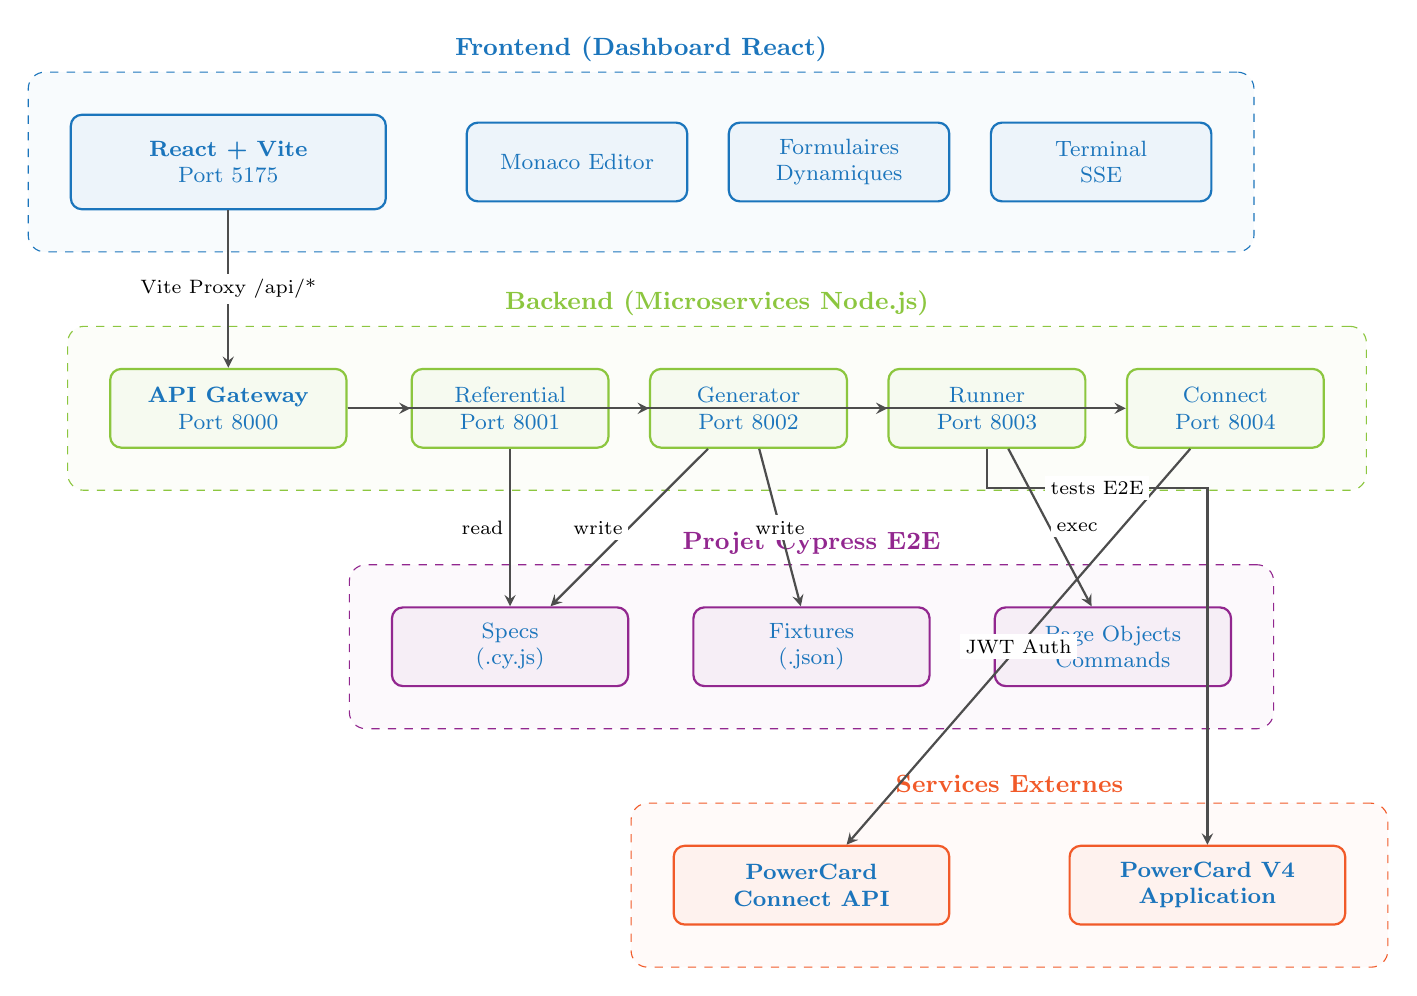
\begin{tikzpicture}[node distance=1.2cm and 1.8cm]
  % ── Frontend Layer ──
  \node[ndBlue, minimum width=4cm, minimum height=1.2cm] (react) {\textbf{React + Vite}\\\footnotesize Port 5175};
  \node[ndBlue, minimum width=2.8cm, right=1cm of react] (monaco) {Monaco Editor};
  \node[ndBlue, minimum width=2.8cm, right=0.5cm of monaco] (forms) {Formulaires\\Dynamiques};
  \node[ndBlue, minimum width=2.8cm, right=0.5cm of forms] (terminal) {Terminal\\SSE};

  \begin{scope}[on background layer]
    \node[bxBlue, fit=(react)(monaco)(forms)(terminal), label={[lB]above:Frontend (Dashboard React)}] (fbox) {};
  \end{scope}

  % ── Backend Layer ──
  \node[ndGreen, minimum width=3cm, below=2cm of react] (gateway) {\textbf{API Gateway}\\\footnotesize Port 8000};
  \node[ndGreen, minimum width=2.5cm, right=0.8cm of gateway] (ref) {Referential\\\footnotesize Port 8001};
  \node[ndGreen, minimum width=2.5cm, right=0.5cm of ref] (gen) {Generator\\\footnotesize Port 8002};
  \node[ndGreen, minimum width=2.5cm, right=0.5cm of gen] (runner) {Runner\\\footnotesize Port 8003};
  \node[ndGreen, minimum width=2.5cm, right=0.5cm of runner] (connect) {Connect\\\footnotesize Port 8004};

  \begin{scope}[on background layer]
    \node[bxGreen, fit=(gateway)(ref)(gen)(runner)(connect), label={[lG]above:Backend (Microservices Node.js)}] (bbox) {};
  \end{scope}

  % ── Cypress Layer ──
  \node[ndPurple, minimum width=3cm, below=2cm of ref] (specs) {Specs\\(.cy.js)};
  \node[ndPurple, minimum width=3cm, right=0.8cm of specs] (fixtures) {Fixtures\\(.json)};
  \node[ndPurple, minimum width=3cm, right=0.8cm of fixtures] (po) {Page Objects\\Commands};

  \begin{scope}[on background layer]
    \node[bxPurple, fit=(specs)(fixtures)(po), label={[lP]above:Projet Cypress E2E}] (cbox) {};
  \end{scope}

  % ── External ──
  \node[ndOrange, minimum width=3.5cm, below=2cm of fixtures] (pwcapi) {\textbf{PowerCard}\\\textbf{Connect API}};
  \node[ndOrange, minimum width=3.5cm, right=1.5cm of pwcapi] (pwcapp) {\textbf{PowerCard V4}\\\textbf{Application}};

  \begin{scope}[on background layer]
    \node[bxOrange, fit=(pwcapi)(pwcapp), label={[lO]above:Services Externes}] (ebox) {};
  \end{scope}

  % ── Arrows ──
  \draw[arw] (react) -- node[lbl]{Vite Proxy /api/*} (gateway);
  \draw[arw] (gateway) -- (ref);
  \draw[arw] (gateway) -- (gen);
  \draw[arw] (gateway) -- (runner);
  \draw[arw] (gateway) -- (connect);
  \draw[arw] (gen) -- node[lbl, left]{write} (specs);
  \draw[arw] (gen) -- node[lbl]{write} (fixtures);
  \draw[arw] (ref) -- node[lbl, left]{read} (specs);
  \draw[arw] (runner) -- node[lbl, right]{exec} (po);
  \draw[arw] (connect) -- node[lbl]{JWT Auth} (pwcapi);
  \draw[arw] (runner.south) -- ++(0,-0.5) -| node[lbl, near start]{tests E2E} (pwcapp);
\end{tikzpicture}
\end{document}
